\chapter[Auto-Adapter Framework]{Auto-Adapter: A Framework for Harness-Validated Robot Driver Synthesis}
\label{chapter:autoadapter-component-analysis}

\begin{quote}\itshape
The objective of this chapter is to present the Auto-Adapter framework and
explain the scope of the evidence it produces. The chapter begins by
introducing the research problem and reviewing the relevant background. It then
describes the framework and its principal stages, presents the experiments and
their results, and discusses the interpretation and limitations of the
resulting evidence. Finally, it
summarises the framework and prepares the basis for the empirical evaluations
that follow.
\end{quote}

\section{Introduction}

Large language models (LLMs) can plan robot actions
\citep{ahn2022saycan,huang2023innermonologue}, but carrying out those plans
requires robot-specific software for motion and observation. Code as Policies
generates robot programmes through supplied APIs
\citep{liang2023codeaspolicies}, while recent agentic systems revise controller
code using execution feedback \citep{tripathi2026testdriven}. This chapter turns
to the robot interface itself: how can its reusable operations and behavioural
tests be generated from task requirements? The resulting driver must then be
evaluated in simulation using observations and verdicts that remain outside its
control.

This chapter presents Auto-Adapter, an LLM-agent framework for generating
robot-specific drivers. It uses public robot documentation, a simulation model
and a task library to define reusable robot operations and their behavioural
requirements. The corresponding tests are generated and fixed before driver
synthesis, without access to the eventual implementation. A coding agent
develops the driver using simulation feedback, while a separate test harness
assesses its behaviour from independently recorded simulator state. We use
ReCAP \citep{zhang2025recap} as the high-level controller to select and compose
these operations for robot task execution.

Here, a capability specifies a reusable robot operation and its expected
behaviour, while a driver provides its robot-specific Python implementation.
For example, \texttt{p \ensuremath{\leftarrow} driver.get\_ee\_position()}
invokes an observation capability, followed by
\texttt{driver.move\_cartesian(p + [0.05, 0, 0])} to invoke a motion capability,
with positions expressed in metres. The driver implements the first call by
reading the robot state and the second by computing and applying actuator
commands.

The empirical objective is to assess whether Auto-Adapter can generate
robot-specific drivers that satisfy defined behavioural requirements and
support downstream robot tasks. Behavioural tests examine whether invoking
each capability through the generated driver produces its specified outcome
in simulation. Task success under ReCAP is assessed separately, preserving
the distinction between implementing robot operations and using them to
complete a task. The practical motivation is to reduce the robot-specific
implementation work required of researchers developing high-level LLM
controllers.

\section{Background}

\subsection{Reusable Robot Capabilities}

Driver synthesis requires a description of the behaviour to be implemented.
A reusable capability expresses an operation that can contribute to several
tasks while leaving their sequencing to a higher-level controller. SkiROS2
illustrates how conditions attached to robot skills support their composition
\citep{mayr2023skiros2}. Code as Policies likewise composes robot programmes
through supplied perception and control APIs \citep{liang2023codeaspolicies}.
For driver synthesis, the further problem is to implement the operations
exposed through such an interface.

A capability therefore needs more than a function signature. For example, a
Cartesian positioning operation must define how its target is interpreted and
what reaching that target means. The same operation can support approaching
an object or positioning a gripper without encoding either complete task.
This motivates deriving reusable operations and their behavioural requirements
from the tasks they must support.

\subsection{Execution-Guided Driver Synthesis}

Implementing an operation requires connecting its intended effect to the
selected robot's control facilities. A positioning request depends on the
robot's joint structure, actuator mapping and coordinate conventions. Errors
in these mappings may produce incorrect motion even when the code executes
without an exception. Execution feedback can therefore inform revisions that
source inspection alone may not resolve. \citet{tripathi2026testdriven}, for
example, refine generated navigation controllers using diagnostics from
structured tests, including evaluation in Webots.

Physics simulation provides a setting in which candidate implementations can
be executed and their effects observed. MuJoCo models articulated dynamics
and contact, allowing control commands to be related to simulated motion
\citep{todorov2012mujoco}. For a positioning operation, an observed trajectory
can reveal whether the end effector approaches the requested target. Such
observations support driver development, while acceptance still requires a
specified behavioural criterion.

\subsection{Independent Behavioural Validation}

Determining whether observed execution satisfies its intended behaviour is
the test oracle problem \citep{barr2015oracle}. For robot drivers, this requires
connecting an operation's specification to an appropriate measurement and
decision rule. A positioning test might measure whether the end effector
reaches a declared tolerance within an allowed interval. A successful return
value alone does not establish that outcome.

This thesis consequently treats independent assessment as a requirement: the
candidate implementation must not control the measurements or acceptance
criteria used to judge it. Requirements must also be justified separately,
since independence cannot correct an inappropriate specification. Passing
capability tests supports behaviour under the tested conditions; completing
a downstream task additionally depends on how operations are selected and
composed. These distinctions motivate separating capability design, driver
implementation and behavioural assessment in the framework that follows. The
resulting simulation evidence does not establish hardware performance.

\section{Auto-Adapter Framework}

\subsection{Framework overview}

Auto-Adapter runs in four phases: study, generate, validation and demo. The
pipeline operates on a working directory containing the robot documentation,
the robot's MJCF model files and a task library.
Figure~\ref{fig:autoadapter-framework-workflow} shows the sequence and the
feedback path from validation to generate.

\textbf{study.} The agent reads the robot documentation and inspects the MJCF
to identify the joints, actuators and control conventions. It records its
findings in \texttt{study.json}, then uses the task requirements to define
reusable operations and their pass criteria. A separate validation compiler
turns these criteria into executable tests before driver generation. The
generation agent receives the capability interface but cannot inspect the
tests. The agent can select a controller skeleton according to the robot's
morphology: damped least-squares (DLS) inverse kinematics (IK) for serial arms,
or proportional--derivative (PD) gait control for quadrupeds.

\textbf{generate.} The agent writes \texttt{driver.py} to implement the required
operations. Through \texttt{execute\_python}, it runs the draft in development
simulations and inspects the resulting robot state and execution errors. It
revises the code against this feedback before submitting the driver to
validation.

\textbf{validation.} The validator checks each capability in fresh MuJoCo
simulations, using simulator state and the pass criteria prepared during study.
For example:
\[
\texttt{driver.move\_cartesian}(\mathbf p^\star),
\qquad
\left\|\mathbf p_{\mathrm{ee}}(T)-\mathbf p^\star\right\|_2
\leq \varepsilon,
\]
where \(\mathbf p^\star\) is the requested target,
\(\mathbf p_{\mathrm{ee}}(T)\) is the end-effector position recorded at the end
of execution, and \(\varepsilon\) is the specified tolerance. If any critical
test fails, generate runs again with the diagnostic messages appended. Each
revised driver is evaluated using the same tests and criteria.

\textbf{demo.} ReCAP uses the generated driver to execute natural-language
tasks, calling only capabilities that passed validation. It observes state
through the driver's high-level methods and plans a sequence of capability
calls, which the runtime executes and logs. For example, a pick-and-place task
involving object \(o\) and target region \(\mathcal G\) follows:
\[
\operatorname{approach}(o)
\rightarrow \operatorname{grasp}(o)
\rightarrow \operatorname{lift}(o)
\rightarrow \operatorname{place}(o,\mathcal G)
\rightarrow \operatorname{release}(o).
\]
The terminal placement condition is
\[
\mathbf p_o(T)\in\mathcal G
\;\land\;
\operatorname{released}(o,T),
\]
where \(\mathbf p_o(T)\) is the object's position at the end of execution.
Success is measured against the task's ground-truth criterion using
independently recorded simulator state and execution video, avoiding reliance
on the controller's self-report.

\textbf{Export.} A passing driver is bundled into
\texttt{auto\_adapter\_\textless robot\textgreater\_artifacts/} together
with the MJCF, the study and validate reports, and a generated README.
Self-contained artifacts run on \texttt{numpy} and \texttt{mujoco} alone.

The following subsections describe robot study and capability design, then
explain how the tests are constructed. They subsequently detail driver
generation, validation and repair, and downstream task execution.

\begin{figure}[htbp]
  \centering
  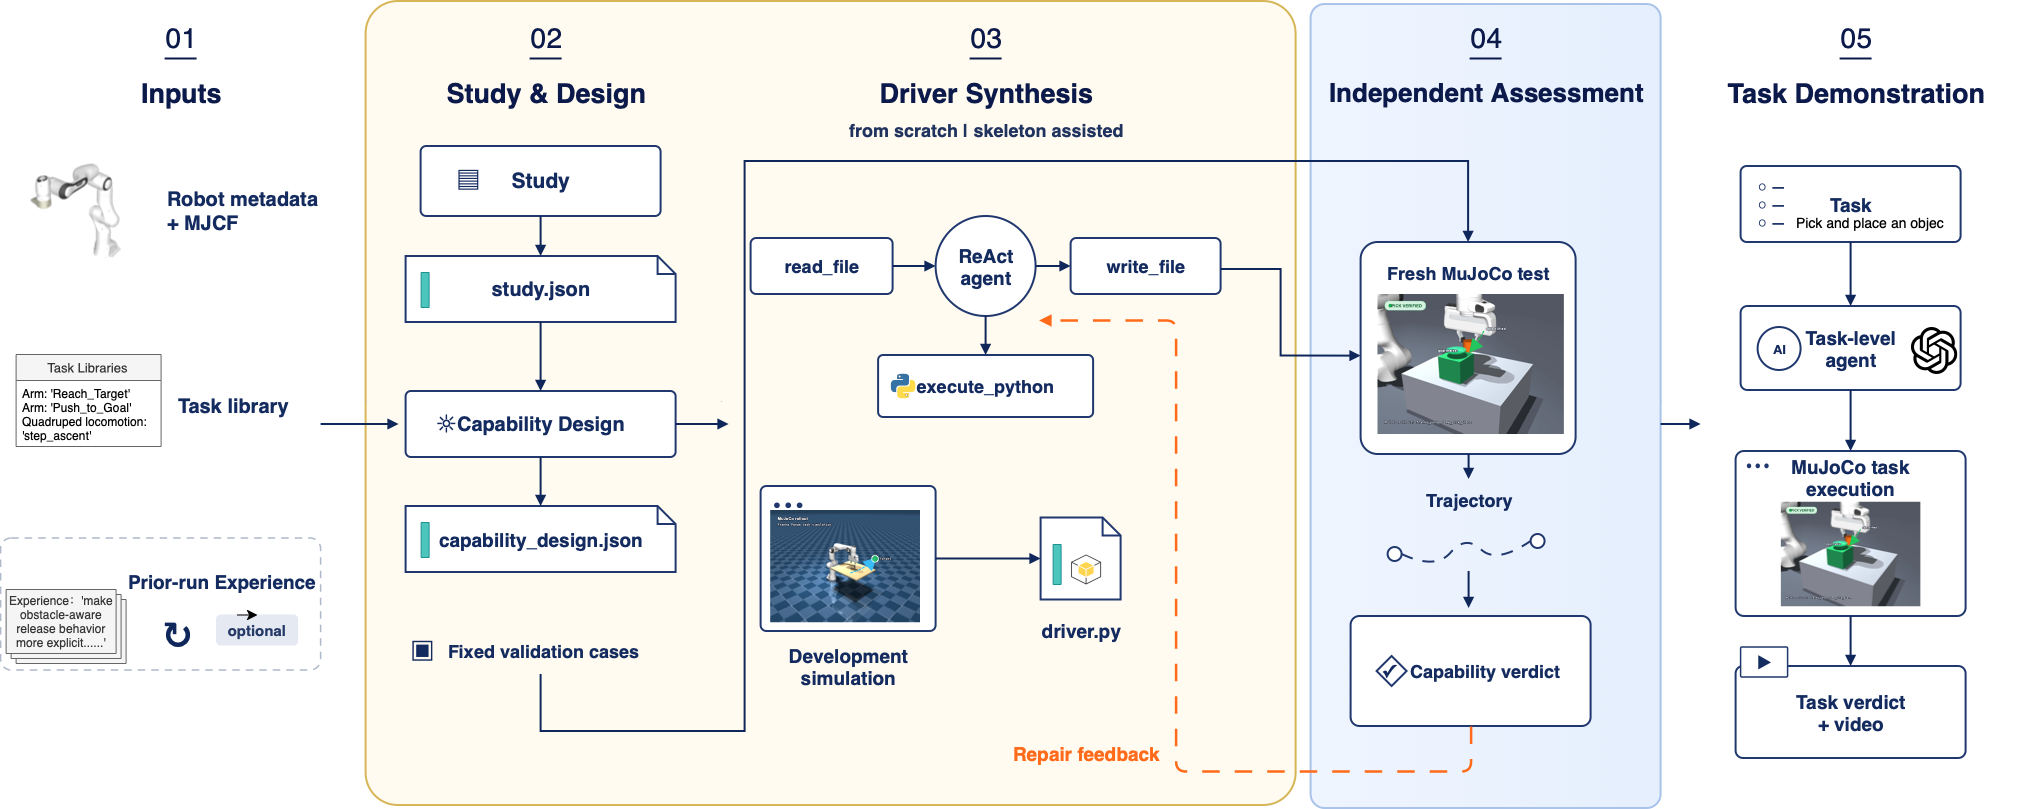
\includegraphics[
    width=\linewidth
  ]{assets/auto_adapter_framework.png}
  \caption[Five-stage Auto-Adapter workflow]
  {Five-stage Auto-Adapter workflow from fixed inputs and capability design to
  driver synthesis, independent MuJoCo assessment, and task demonstration. The
  dashed path denotes bounded Repair feedback.}
  \label{fig:autoadapter-framework-workflow}
\end{figure}

\subsection{Task-Grounded Capability and Validation Design}

The design agent uses the task library and robot study to determine which
operations the driver must expose. It groups task requirements that share a
physical effect or observation. For example, approaching an object and
reaching a placement location both require end-effector positioning. These
destinations become a target parameter, while the task controller selects and
orders targets. The design records which tasks motivate each capability.

The capability contract specifies the request, promised behaviour and
operating range. For Cartesian positioning, it identifies the coordinate
frame, units and end-effector reference. A reach-and-hold request requires
\[
e_k=\left\|\mathbf p_{\mathrm{ee}}(t_k)-\mathbf
p^\star\right\|_2\leq\varepsilon
\]
at consecutive simulation steps spanning at least \(\tau\) and ending by
\(T_{\max}\). Here, \(\mathbf p^\star\) is the requested target and \(\mathbf
p_{\mathrm{ee}}(t_k)\) is the measured position of the declared reference. The
time \(t_k\) is measured from invocation at simulation step \(k\), and
\(\varepsilon\) is the position tolerance. The minimum holding duration
\(\tau\) rejects a brief crossing of the target region. The deadline
\(T_{\max}\) uses the same time origin as \(t_k\).

These numerical parameters are set before driver synthesis, retaining explicit
task requirements for accuracy and duration. Where values are absent, the LLM
proposes them and records their justification against the task and documented
operating conditions. The proposals require examination during validation
design because geometry and joint limits alone do not determine acceptable
task accuracy.

A separate validation compiler translates each contract into executable cases.
Each case combines an initial simulation state, a concrete request and
bindings between observations and MuJoCo entities. For reaching, the compiler
samples the body or site representing the declared end-effector reference and
applies the error and timing conditions. Each capability receives a nominal
case and a feasible case near its declared operating boundary. An
independently prepared reference implementation must pass both cases before
the suite is fixed. This establishes feasibility for those cases, without
establishing that the suite rejects every incorrect implementation.

\subsection{Driver Synthesis and Validation}

The coding agent implements the capability contracts in \texttt{driver.py}.
From-scratch synthesis generates control code, while skeleton-assisted
synthesis configures a supplied controller and exposes the required methods.
Robot bindings map joint names to position and velocity addresses, and
actuator names to control indices. For the supplied serial-arm skeleton, the
velocity addresses also select the corresponding columns of the positional
Jacobian. Separate mappings accommodate differences in joint ordering,
actuator ordering and the dimensions of the position and velocity arrays.

For serial arms, the supplied controller uses DLS inverse kinematics
\citep{wampler1986inverse}. The solver computes a joint target through
kinematic evaluations and restores the original configuration before
execution. The driver then interpolates position commands from the current
control targets through \texttt{data.ctrl}, advancing MuJoCo at each step.
During development, the agent compares the executed end-effector position with
the requested target and inspects execution errors. This feedback guides
revisions to robot bindings, control settings or execution duration.

For each validation case, the harness creates a fresh MuJoCo model and
simulation state. It binds the driver to these objects before establishing the
prescribed initial state. The checker reads observations directly from the
simulation and applies the compiled acceptance conditions. For motion
capabilities, acceptance requires actuator commands and physics steps to
produce the evaluated motion; numerical pose assignments cannot substitute for
that trajectory.

Failures return diagnostics for bounded repair, while executable checkers and
the reference implementation remain withheld from the coding agent. The
harness evaluates each revised driver against the original cases and criteria.
Capabilities passing both cases become available to ReCAP through
contract-derived tool schemas specifying operation names and argument types.
Wrappers convert structured arguments into driver calls, including assembling
Cartesian coordinates into a target vector. A separate task-level criterion
evaluates the outcome produced by the selected calls.


\section{Experiments and Results}

\subsection{Experimental Configuration}

Experiment 1 covers eleven robot configurations. These are SO-101, Unitree
Go2, Franka Panda, Kinova Gen3, xArm7, UR5e, Piper, KUKA iiwa 14, LEAP Hand,
Stretch 2 and ALOHA 2. Each configuration is evaluated in three fresh runs,
giving 33 experimental units.

Figure~\ref{fig:robot-platform-taxonomy} presents fifteen robot platforms grouped by embodiment type. Experiment 1 uses the eleven configurations listed above.

\begin{figure}[htbp]
  \centering
  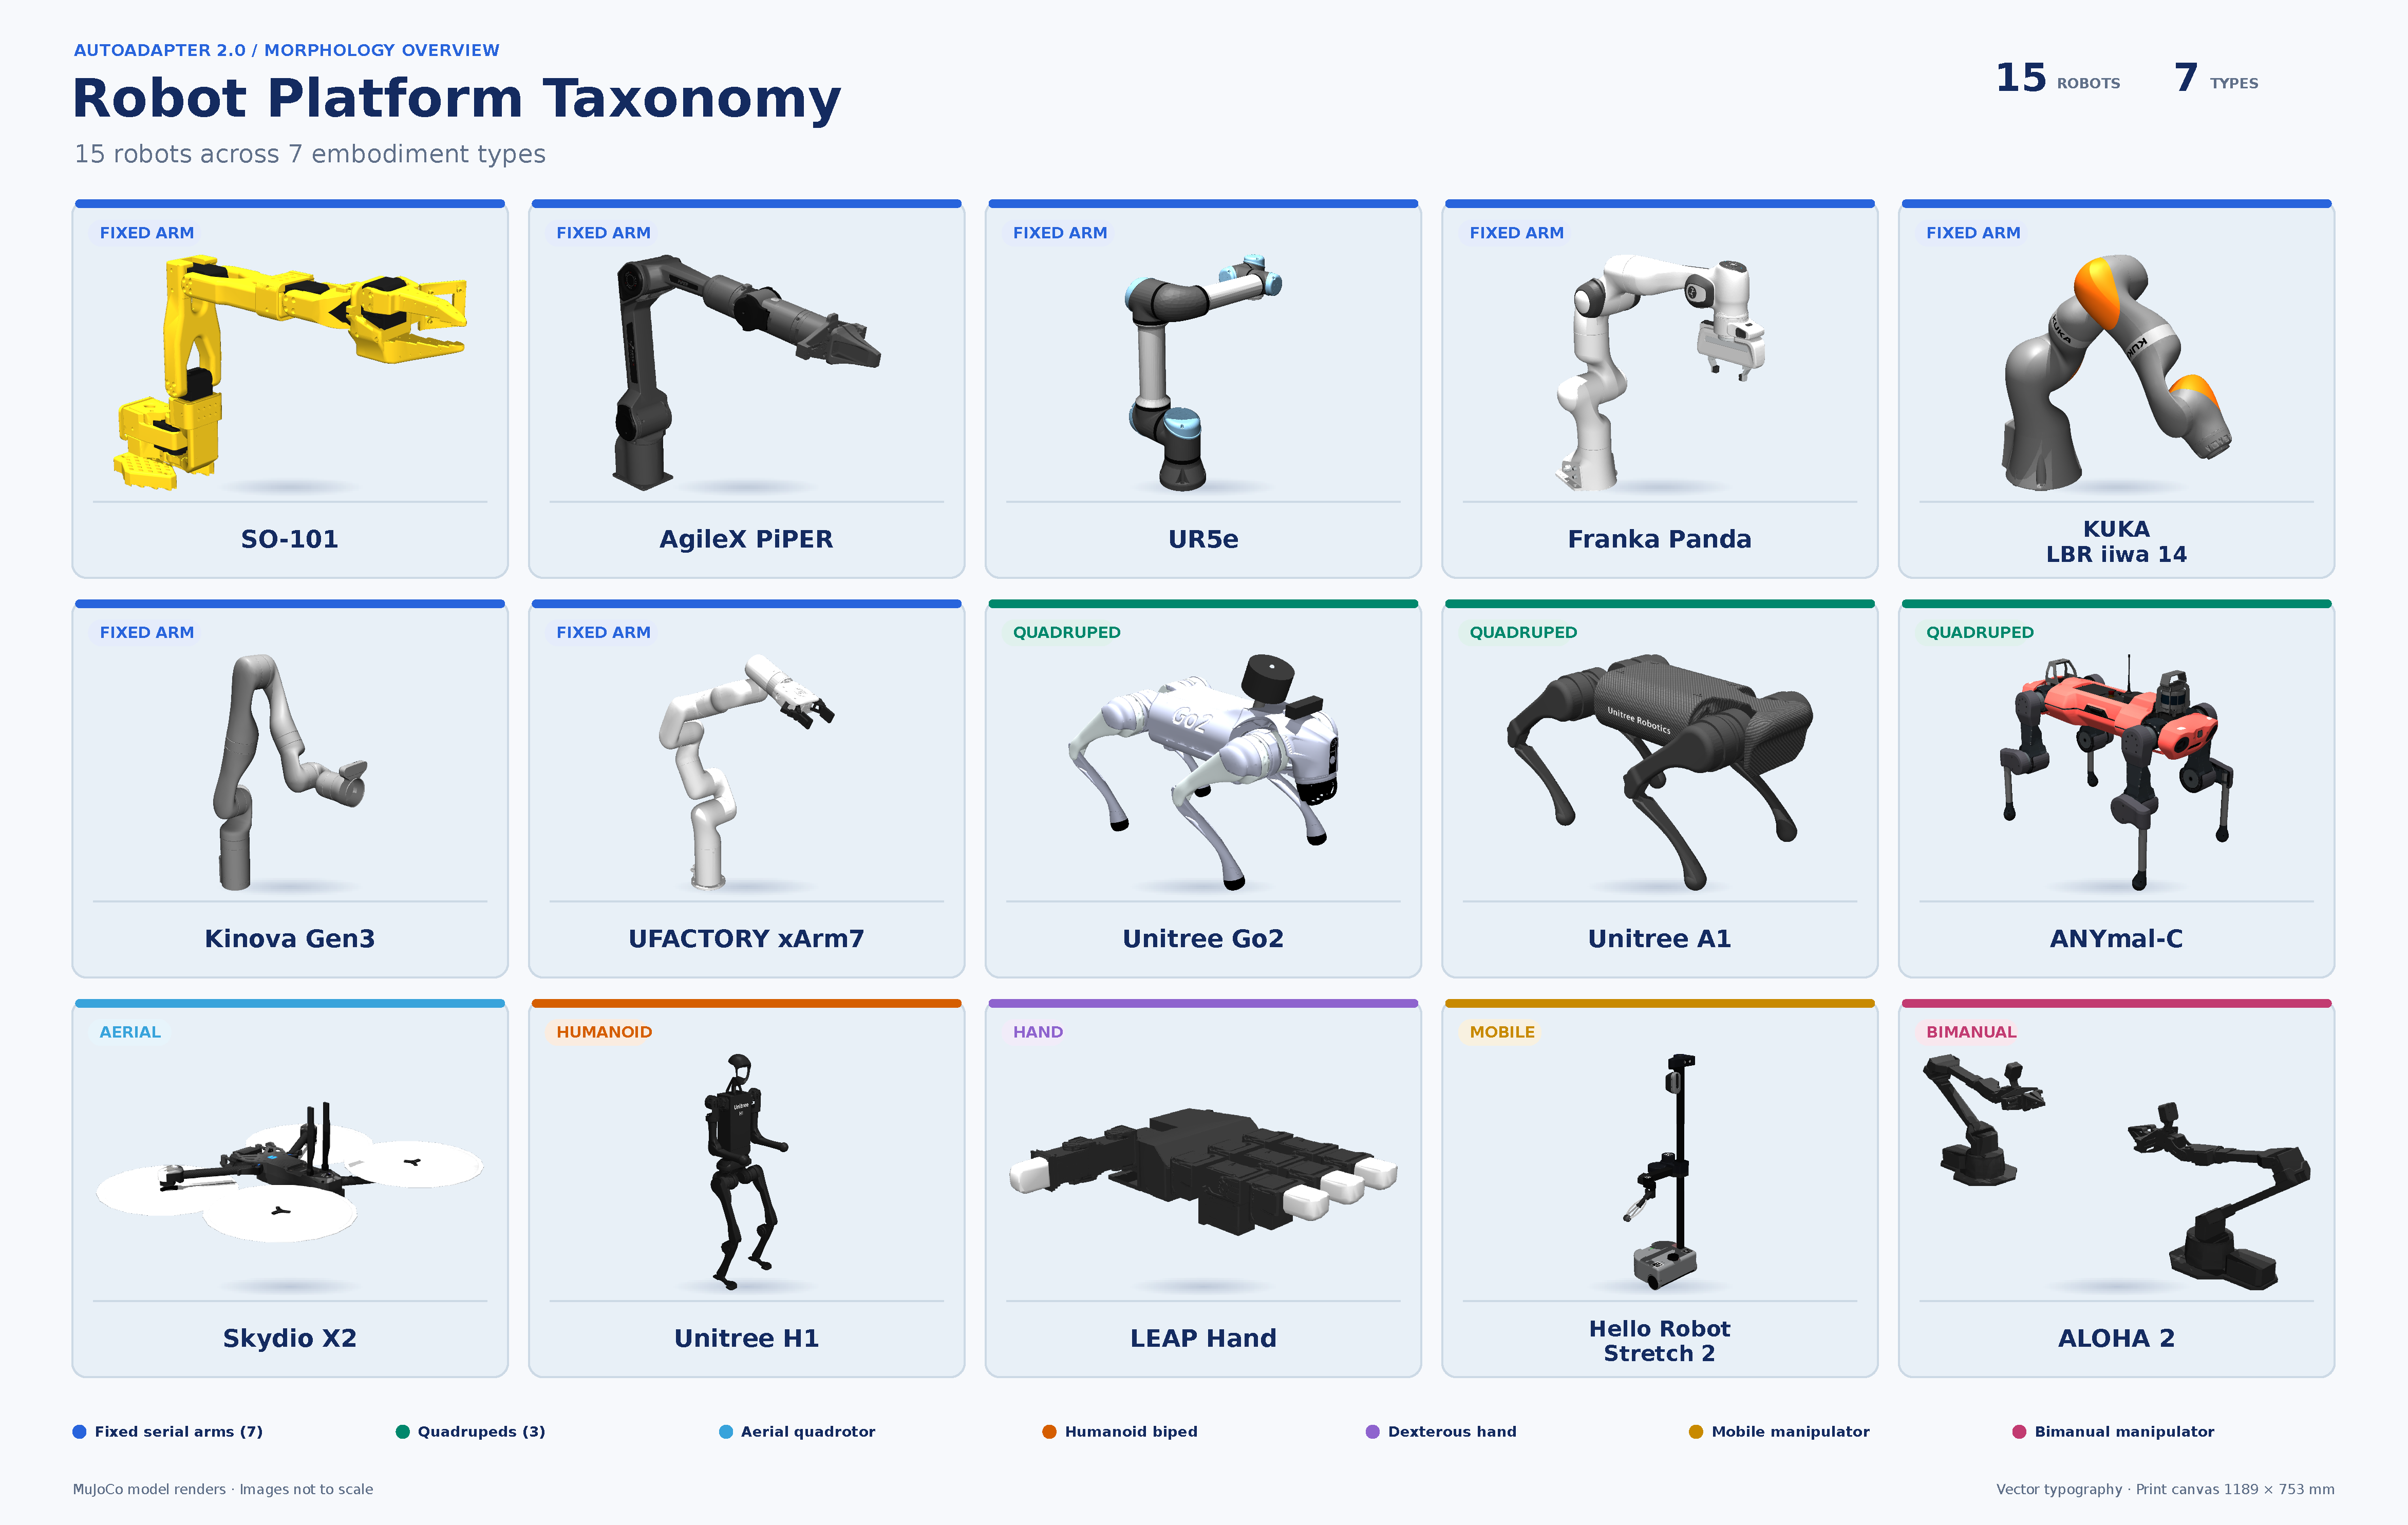
\includegraphics[width=\linewidth]{assets/robot_platform_taxonomy_15_print.pdf}
  \caption[Fifteen robot platforms grouped into seven embodiment types]
  {Fifteen robot platforms grouped into seven embodiment types.
  \textbf{Fixed arms:} SO-101, AgileX PiPER, UR5e, Franka Panda, KUKA LBR iiwa 14,
  Kinova Gen3 and UFACTORY xArm7.
  \textbf{Quadrupeds:} Unitree Go2, Unitree A1 and ANYmal-C.
  \textbf{Aerial quadrotor:} Skydio X2.
  \textbf{Humanoid biped:} Unitree H1.
  \textbf{Dexterous hand:} LEAP Hand.
  \textbf{Mobile manipulator:} Hello Robot Stretch 2.
  \textbf{Bimanual manipulator:} ALOHA 2.}
  \label{fig:robot-platform-taxonomy}
\end{figure}

\begin{table}[htbp]
  \centering
  \caption{Robot platforms grouped by embodiment type.}
  \label{tab:robot-platform-embodiment-types}
  \small
  \renewcommand{\arraystretch}{1.15}
  \begin{tabularx}{\linewidth}{@{}l>{\raggedright\arraybackslash}X@{}}
    \toprule
    \textbf{Robot type} & \textbf{Robot platforms} \\
    \midrule
    Fixed serial arm & SO-101; AgileX PiPER; UR5e; Franka Panda; KUKA LBR iiwa 14; Kinova Gen3; UFACTORY xArm7 \\
    Quadruped & Unitree Go2; Unitree A1; ANYmal-C \\
    Aerial quadrotor & Skydio X2 \\
    Humanoid biped & Unitree H1 \\
    Dexterous hand & LEAP Hand \\
    Mobile manipulator & Hello Robot Stretch 2 \\
    Bimanual manipulator & ALOHA 2 \\
    \bottomrule
  \end{tabularx}
\end{table}

All runs use Claude Sonnet 4.6 under the same skeleton-assisted generation
condition and execution limits. Within each robot, the task, capability design,
simulation assets and private validation suite remain unchanged. Every run uses
a fresh model conversation, workspace and simulator reset. No information is
transferred between runs.

The validation suites define 58 capabilities and 116 test cases. A test case
invokes one capability with specified inputs from a fixed initial state. An
independent evaluator measures the resulting state and motion in the physics
simulator. It then applies a numerical pass criterion. Each capability has two
cases: one representative request and one request near its permitted operating
limit.

A driver qualifies only if all its test cases pass. Capabilities that pass both
cases are made available for task execution. If none passes, the task is
recorded as not run. Task success is reported separately from complete-driver
qualification.

All 33 runs remain in the denominator. Early termination is reported with its
stage and reason. Results are summarised for each robot and for the experiment
as a whole. The analysis is descriptive because the tasks and simulation
environments differ between robots.


\subsection{Results}

\section{Interpretation and Limitations}

Auto-Adapter's principal methodological choice is to separate capability
design, driver implementation, and behavioural judgement. Task-Grounded
Capability Design connects a task-neutral interface to source-backed task
requirements, while the Independent Validation Compiler defines executable
cases without access to candidate code. The trusted \emph{Harness} then applies
fixed criteria to measurements recorded outside the candidate. This arrangement
prevents driver return values and self-reported completion from determining
acceptance. It does not remove judgement from translating task standards into
capability criteria or make the resulting suite exhaustive.

The evidence produced at each stage answers a different question. Source and
import checks establish only that a candidate can be loaded. A Capability
Validation pass supports the declared physical effect for the exact nominal and
calibrated-boundary cases; those two cases do not cover every request,
interaction, or long-horizon composition. A Task Demo evaluates downstream
composition using only capabilities that passed both cases. Its outcome neither
changes the earlier capability verdicts nor establishes that the complete
driver passed. Similarly, a terminal pass after Repair measures performance
after bounded feedback and must remain distinct from initial-attempt
performance.

The framework definition alone does not establish that Auto-Adapter reliably
produces effective drivers, outperforms alternative methods, or generalises
across robot configurations. Those questions require the controlled
evaluations in later chapters. Furthermore, Direct-MuJoCo evidence is
conditional on the selected assets, requests, initial states, observation
operators, and thresholds. It does not measure real-SDK fidelity, sensing
uncertainty, communication latency, calibration error, hardware safety, or
sim-to-real transfer. Cross-configuration outcomes must remain descriptive
because morphology, actuation, task catalogue, scene, and observation
facilities vary together.

\section{Summary}

This chapter defined Auto-Adapter as a framework for constructing a reusable,
robot-specific Python driver from public robot information and source-backed
task requirements. It first studies the robot and fixed simulation model,
derives task-neutral capabilities, and compiles implementation-blind
behavioural cases. A bounded ReAct coding agent then implements the driver
using public MuJoCo feedback. The trusted \emph{Harness} evaluates the
resulting actuator-mediated trajectories against fixed criteria rather than
relying on candidate output.

The workflow keeps source checking, capability validation, Repair, downstream
Task Demo, and any later Experience use distinct. Only capabilities satisfying
both their nominal and calibrated-boundary cases are exposed to Task Demo, and
its terminal outcome does not rewrite driver verdicts. These boundaries provide
an auditable basis for empirical comparison; they are not themselves evidence
of universal integration or hardware readiness.
Chapter~\ref{chapter:autoadapter-bench} evaluates driver synthesis and
downstream use under controlled inputs, while
Chapter~\ref{chapter:cross-robot-evaluation} examines the complete construction
route across the declared Direct-MuJoCo configurations.
